\section{Project Objectives}
The key innovation in the approach that DEIS takes to address the dependability problem of CPS, is the concept of Digital Dependability Identity (DDI), which was outlined by key partners of DEIS in \cite{}. 
In general, a Digital Identity is defined as \emph{the data that uniquely describes a person or a thing and contains information about the subject's relationships} \cite{}. 
To this extent, it contains all attributes that characterise an object, how the object can be accessed, who can access the object, and how it may interact with other objects. In addition, a DDI contains all the information that uniquely describes the dependability characteristics of a system or component. This includes two key aspects: (a) attributes that describe the system’s or component’s dependability behaviour, such as faults and possible fault propagations through the CPS architecture, which can be described using concepts from the theory of safety contracts; and (b) requirements on how the component interacts with other entities in a dependable way, described in terms of the level of trust and assurance.

A DDI is therefore an evolution of current modular dependability assurance models of a system. It is produced during design, issued when the component is released, and then continuously maintained over the complete lifetime of a component or system. DDIs are used for the integration of components into systems during development as well as for the dynamic integration of systems into \emph{systems of systems} in the field. The main difference in the two cases lies mainly in the degree of automation that integration of DDIs requires: for instance, while a manual process might be sufficient to ensure dependability requirements are met at the integration interface between silicon providers and first-tier suppliers, the dynamic integration of systems of systems in the field requires a fully automated evaluation of DDIs in order to ensure a dependable collaboration.

It is obvious that a DDI is potentially a very useful digital artefact - it is a living dependability assurance case, the utility of which spans from component design to in-the-field operation of a CPS. However, the production and use of DDIs for heterogeneous systems poses a number of significant technological and engineering challenges that are pertinent and important in industry today and motivate the objectives of this project. 

\subsection{Challenge 1. Universal exchange of dependability information}
It is expected that DDIs will be produced by multiple stakeholders in a supply chain. They therefore need to be interoperable and expressed in a common communication language that can be understood by stakeholders and mechanisms undertaking the generation and evaluation of DDIs. Currently, there is a lack of a common model for the exchange of dependability information. Thus, a precondition for DDI is the existence of an open dependability metamodel, which can provide the basis for expressing DDIs. 

In addition to the open meta-model, for DDIs to be an effective means for synthesis of heterogeneous dependability information, they must be sufficiently expressive to enable the component integrator to compile DDIs from the DDIs of sub-components. Moreover, DDIs should optionally shield sensitive details through abstraction to protect the component provider’s Intellectual Property. 

\subsection{Challenge 2. Efficient dependability assurance across industries and value chains}
In current industrial practice, different dependability tools and methodologies are used. For practicality and to increase uptake of new specifications such as the proposed DDI, it must be possible for a component provider to generate DDIs based on the information that is already available in the tools that are established in a company. Moreover, it must be possible to include the information contained in DDIs into the established dependability assurance lifecycle and tool chain of the component integrator. 

In a typical scenario, system and component requirements and their integration context change constantly; these changes need to be reflected in the dependability analyses of a system. This in turn requires the ability to perform semi-automated change-impact analyses across the DDIs of components to reflect design changes in a system DDI. As a further aspect, it is typical for companies to develop product families instead of single products. For example, in the automotive industry, it is not unusual to assure the safety of more than a thousand variants of a powertrain control system per year. This requires that DDIs support variability, including analyses that enable a prediction about whether a component will fit into all product variants, or which constraints should be considered in the definition of the product family in order to avoid expensive re-assurance effort.

Finally, there is the challenge of how to manage dependability from the early stages of design, so that it is not treated as an emergent property. This is important for the synthesis of DDIs, because controlled processes with rational allocation of requirements that can work across the tiers of a value chain can also assist in the effective collection and synthesis of DDIs. Numerous safety standards in various industries, such as the generic safety standard IEC61508 and the more relevant automotive safety standard ISO26262, envisage controlled processes of design refinement which are driven by safety requirements typically expressed as Safety Integrity Levels. These processes implicitly define similar patterns for the construction of dependability assurance cases that ideally should be captured so that their model-based, and automated where possible, synthesis can then become possible. Note that all these are significant challenges in current certification not only of CPS but complex embedded systems in general.  


\subsection{Challenge 3. Dependable integration of systems in the field}

In CPS, dependability cannot be fully assured prior to deployment. Indeed, systems will dynamically interconnect and form systems of systems with largely unpredictable consequences for dependability. In order to assure the dependability of such in-field integrations, the degree of automation in the evaluation of DDIs must be further increased to include additional forms of runtime or in-the-field evaluation that will enable or disable operations in a particular configuration or context. DDIs therefore must become executable specifications, not simply digital artefacts that cease in their utility after deployment of the system.  

First, DDIs must be made publicly available, e.g. in a (secure) registry residing in the cloud, to all companies whose systems shall be integrated into a particular CPS, so that developers of new systems can check whether their system can be integrated in a dependable way. Companies shall have the possibility to stay informed about changes in an CPS family in order to check if this requires modifications in their systems. For highly dynamic environments, it is additionally necessary to enable a fully automated evaluation of DDIs so that it is possible to decide, either without human interaction or via a decision support system, whether or not a dependable collaboration is possible. Such a check based on the system DDIs should be possible off-board (e.g., in the cloud) as well as on-board, in the latter case with the DDIs as executable specifications and being evaluated by the systems themselves.

%\begin{enumerate}
%	\item \textbf{Universal exchange of dependability information}
%	\item \textbf{Efficient dependability assurance across industries and value chains}
%	\item \textbf{Dependable integration of systems in the field}
%\end{enumerate}

\begin{figure}[ht!]
	\centering
	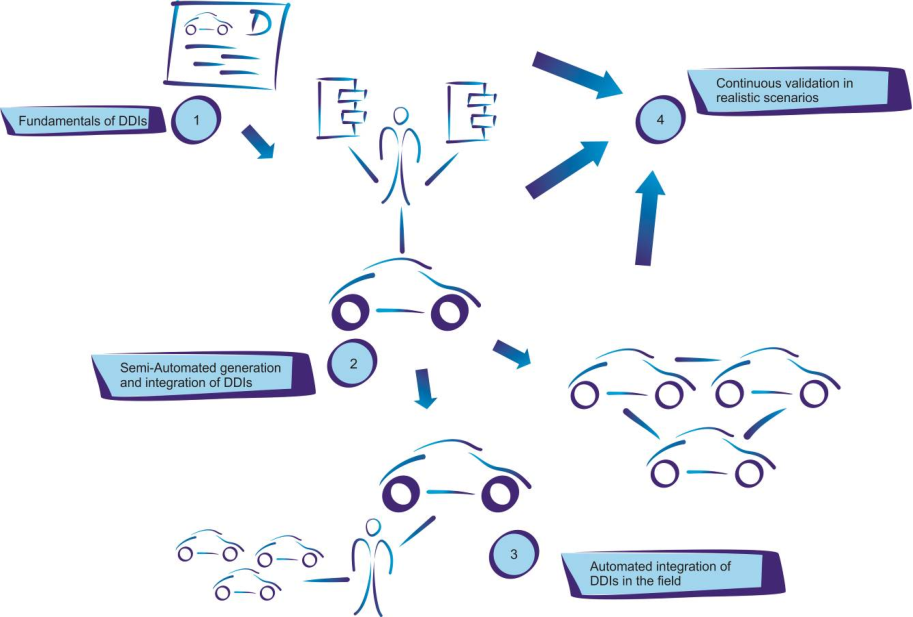
\includegraphics[width=1\linewidth]{./fig/proj_concept.pdf}
	\caption{DEIS project concept}
	\label{fig:proj_concept}
\end{figure}


